\documentclass[intlimits, 9pt, unicode]{beamer} 

\usepackage[T2A]{fontenc}
%\usepackage[cp1251]{inputenc}
\usepackage[utf8]{inputenc}
\usepackage[russian]{babel}
\usepackage{graphicx}
\usepackage{amssymb}
\usepackage{amsthm}

\usefonttheme[onlymath]{serif}

\usepackage{beamerthemesplit}

\usetheme{Warsaw}

\setbeamerfont{institute}{size=\normalsize}

\setbeamercolor{bluetext_color}{fg=blue}
\newcommand{\bluetext}[1]{{\usebeamercolor[fg]{bluetext_color}#1}}

\setbeamercovered{transparent}

\title{Change point detection in mobile advertising}
\author{Nina Golyandina, Kliment Merzlyakov}
\institute{Saint Petersburg State University \\
    Mathematical faculty \\
     Applied statistics department \\
}
\date{
    Saint Petersburg\\
    2018
}

\begin{document}

\begin{frame}
    \titlepage
\end{frame}

\begin{frame}
    \frametitle{Content}

    \begin{itemize}
    	\item Change point detection
		     	 \begin{itemize}
	    		   \item What is change point detection?
		    	   \item Real world examples of change point detection 
		    	   \item Reasons to detect change points
		    	  \end{itemize}
        \item Change point detection techniques
        \item Airpush cases
		     	 \begin{itemize}
	    		   \item Fraud elimination
		    	   \item Trend extraction
		    	   \item Smart alerts
		    	  \end{itemize}
    \end{itemize}
\end{frame}


\begin{frame}
    \frametitle{What is change point detection?}

    \begin{itemize}
    	\item Change point --- point in time series where some significant change occurred
	\item Change point detection --- group of methods to find change points in time series
    \end{itemize}
\end{frame}

\begin{frame}
    \frametitle{Types of change points}

    \begin{itemize}
    	\item Trend change
	\item Mean change
	\item Variance change
	\item Single point change
	\item Period change
	\item Structure change
    \end{itemize}
\end{frame}

\begin{frame}
\frametitle{Change point examples}
\begin{figure}
\textbf{Common graph}\par\medskip
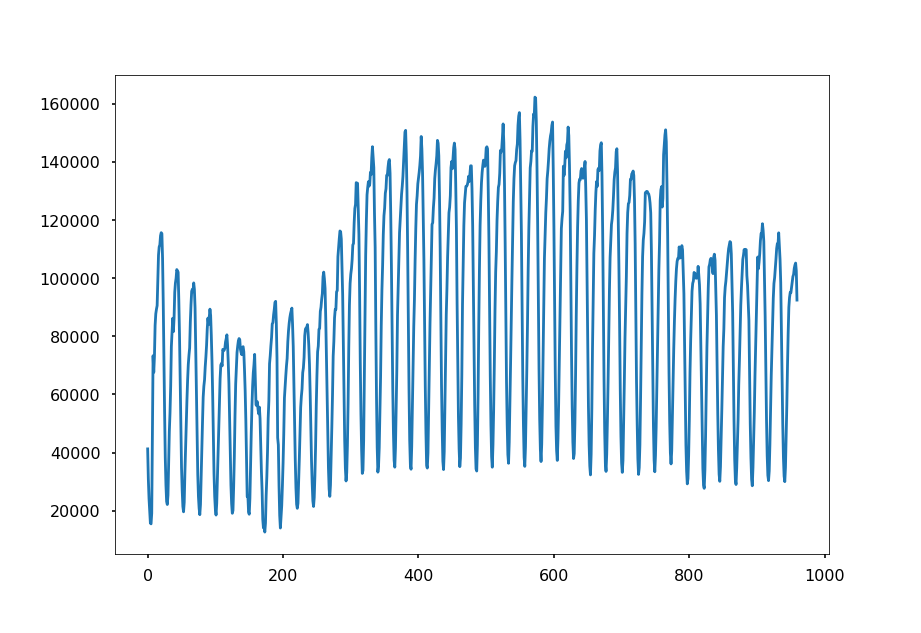
\includegraphics[scale=0.30]{images/001_normal_1}
\end{figure}
\end{frame}

\begin{frame}
\frametitle{Change point examples}
\begin{figure}
\textbf{Common graph with trend}\par\medskip
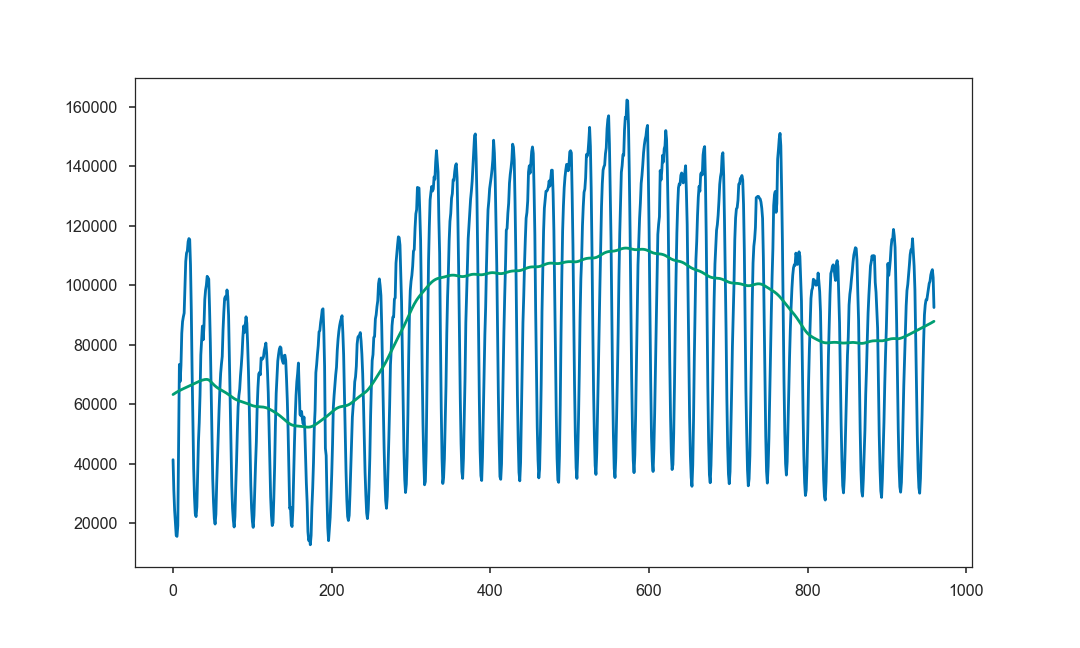
\includegraphics[scale=0.30]{images/001_normal_2}
\end{figure}
\end{frame}

\begin{frame}
\frametitle{Change point examples}
\begin{figure}
\textbf{Common graph without trend}\par\medskip
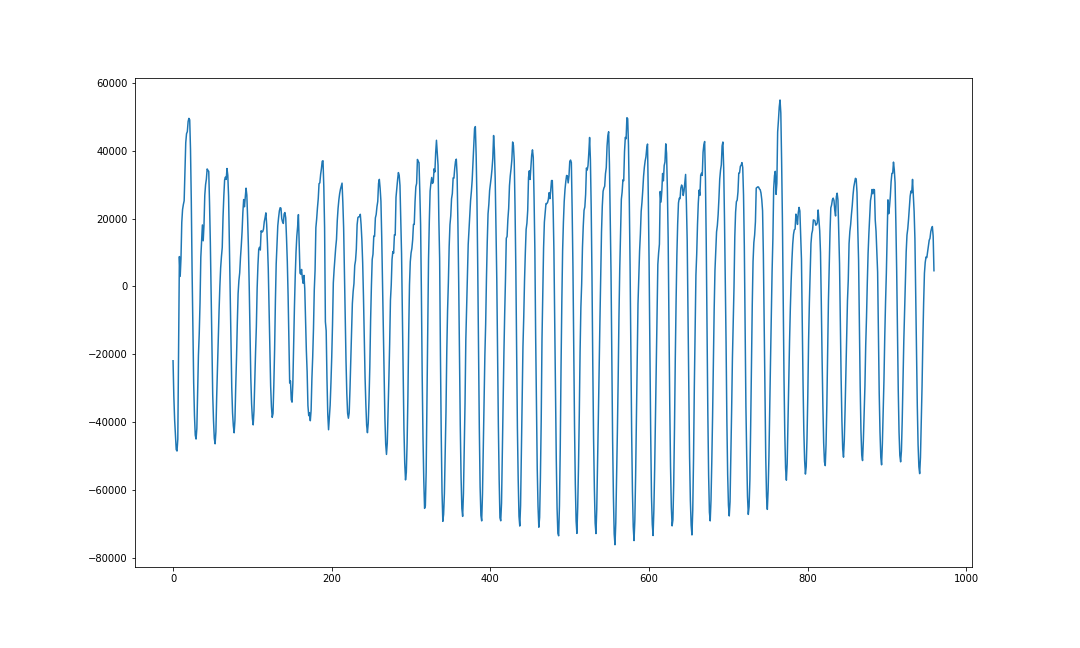
\includegraphics[scale=0.30]{images/001_normal_3}
\end{figure}
\end{frame}

\begin{frame}
\frametitle{Change point examples}
\begin{figure}
\textbf{Common graph periodic frequency}\par\medskip
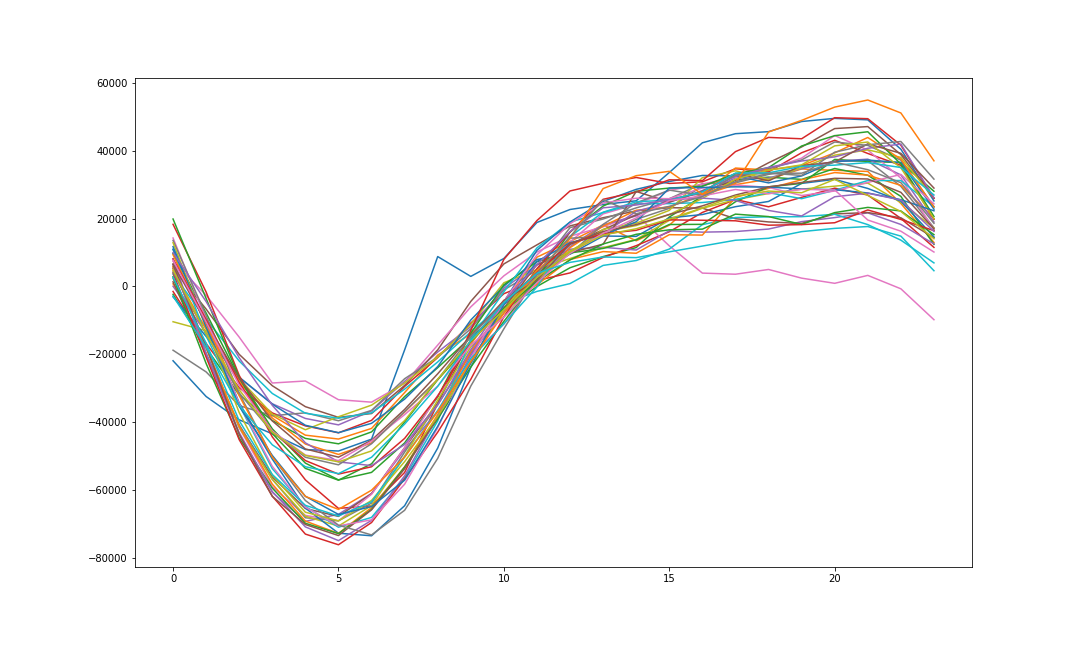
\includegraphics[scale=0.30]{images/001_normal_4}
\end{figure}
\end{frame}

\begin{frame}
\frametitle{Change point examples}
\begin{figure}
\textbf{Mean change}\par\medskip
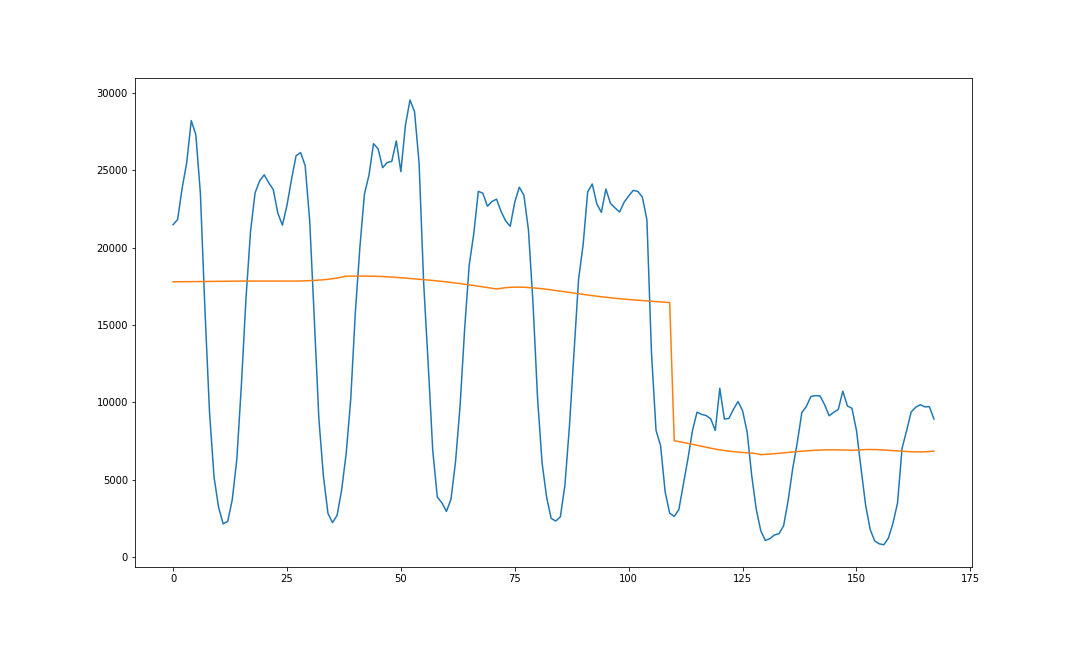
\includegraphics[scale=0.30]{images/002_mean}
\end{figure}
\end{frame}

\begin{frame}
\frametitle{Change point examples}
\begin{figure}
\textbf{Variance change}\par\medskip
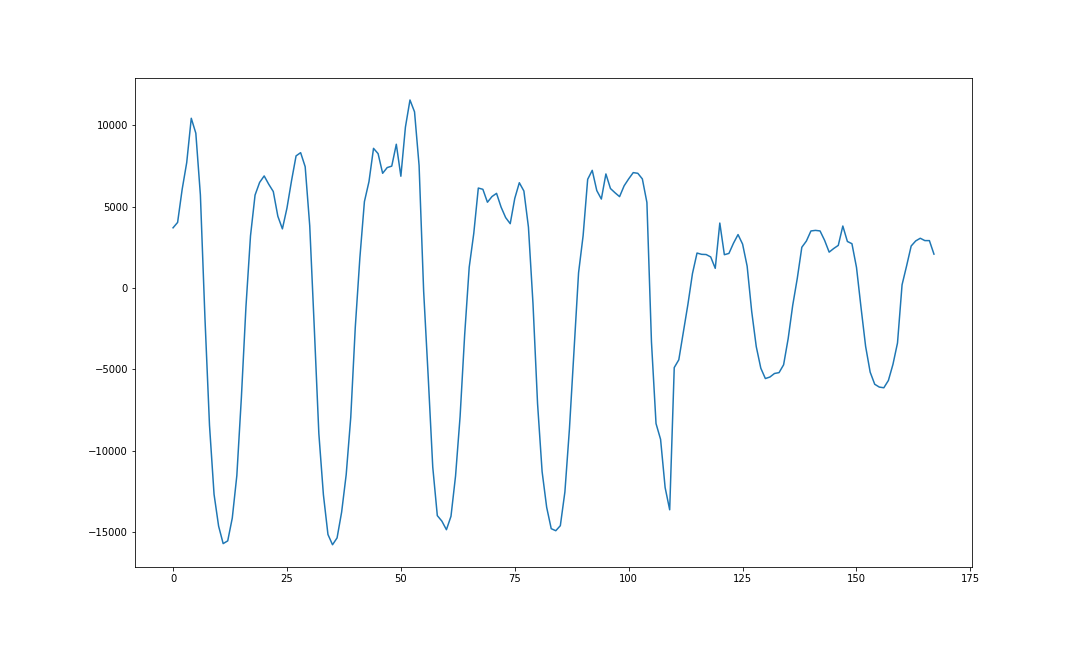
\includegraphics[scale=0.30]{images/003_variance}
\end{figure}
\end{frame}

\begin{frame}
\frametitle{Change point examples}
\begin{figure}
\textbf{Trend change}\par\medskip
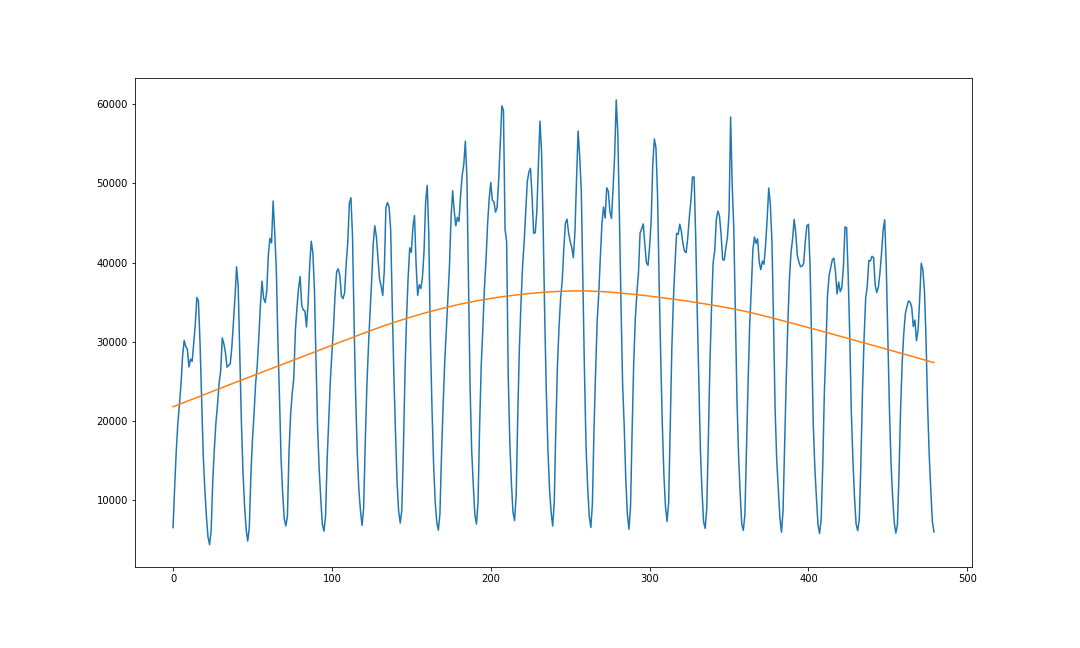
\includegraphics[scale=0.30]{images/004_trend}
\end{figure}
\end{frame}

\begin{frame}
\frametitle{Change point examples}
\begin{figure}
\textbf{Point change}\par\medskip
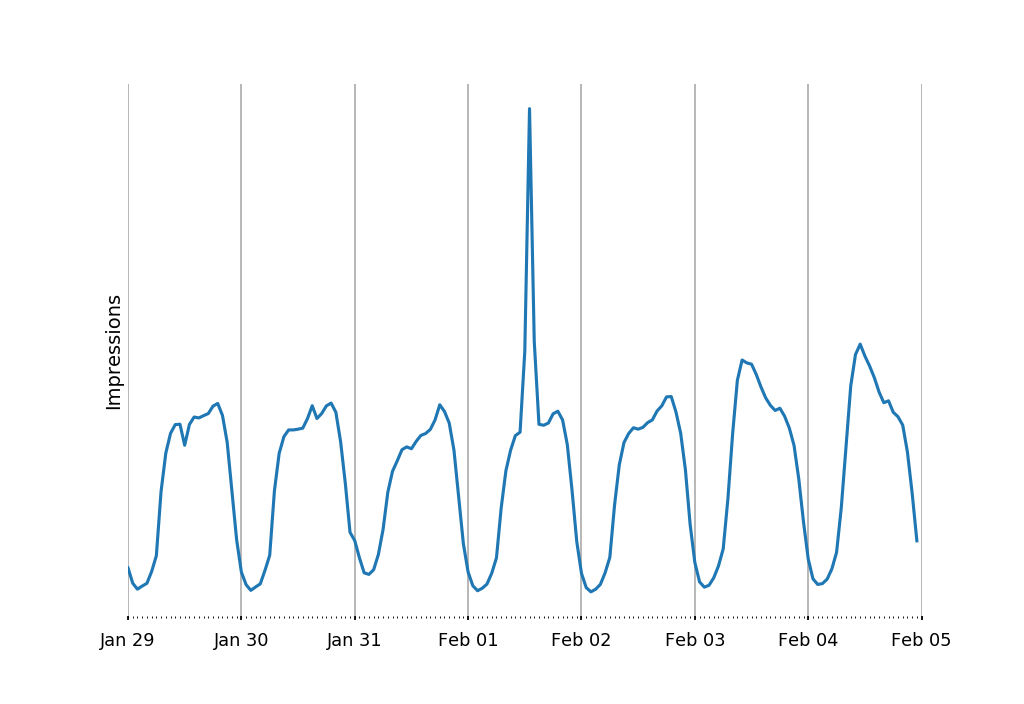
\includegraphics[scale=0.30]{images/005_point}
\end{figure}
\end{frame}

\begin{frame}
\frametitle{Change point examples}
\begin{figure}
\textbf{Structure change}\par\medskip
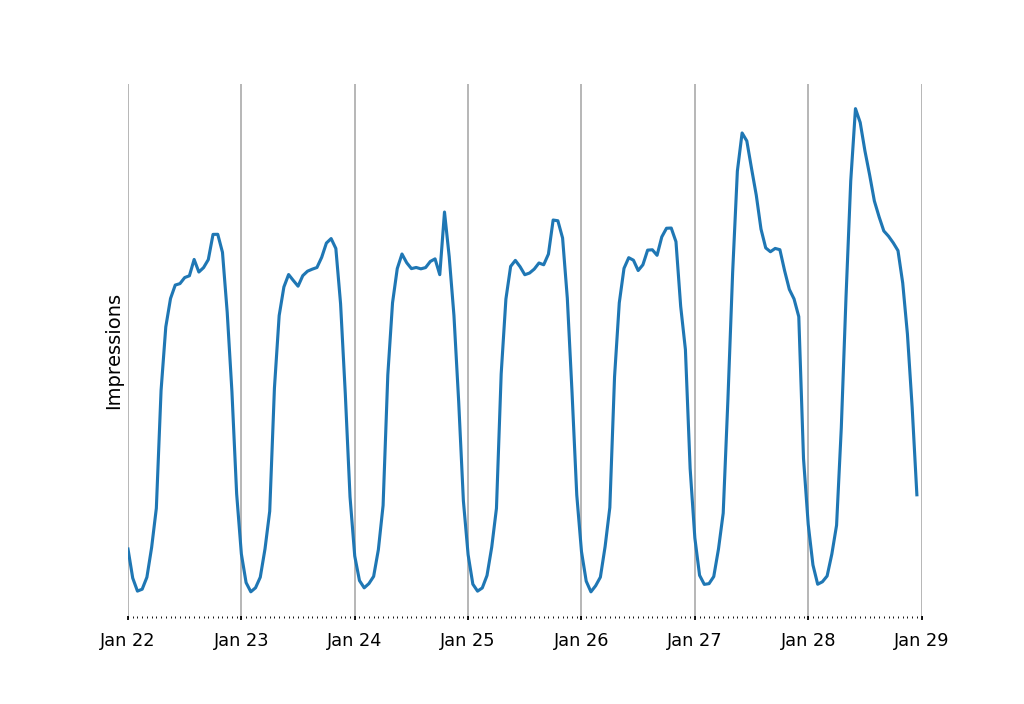
\includegraphics[scale=0.30]{images/006_structure}
\end{figure}
\end{frame}

\begin{frame}
    \frametitle{Reasons to detect change points}

    \begin{itemize}
    	\item Searching issues in historical data 
	\item Reacting on changes quickly
	\item Extracting trend more accurately
    \end{itemize}
\end{frame}



\begin{frame}
    \frametitle{Airpush cases. Fraud elimination}
    \begin{itemize}
    	\item Apps minutely requests data
	\item Red flag: strong pattern.
	\item Can be a automated bots behind pattern
    \end{itemize}
    \begin{figure}
	\textbf{Clean application}
	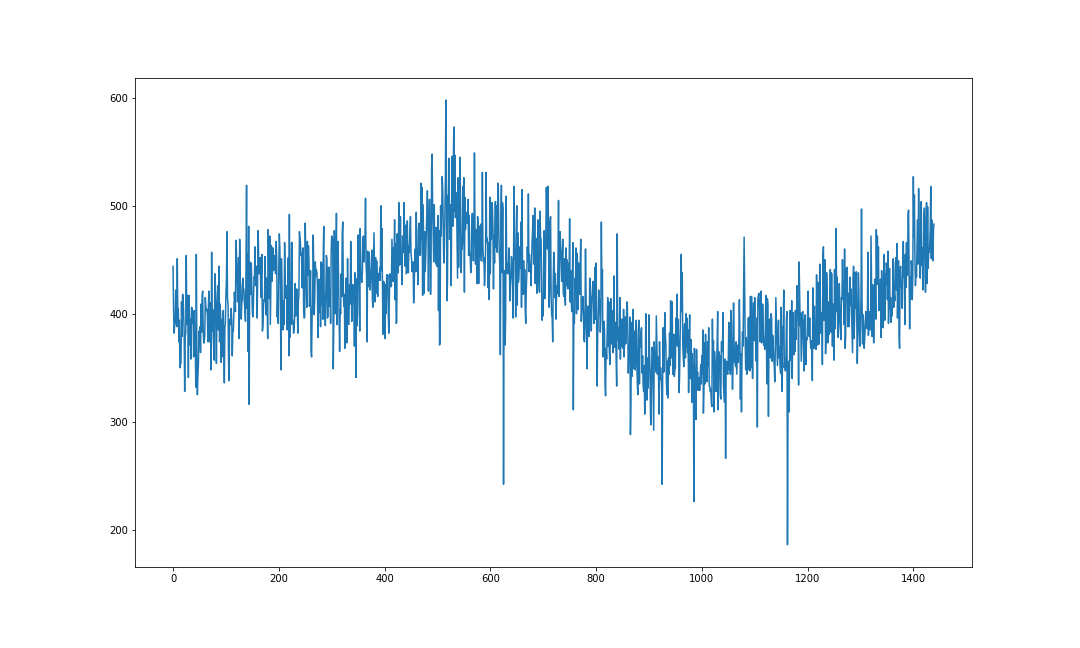
\includegraphics[scale=0.10]{images/007_case_1}
	\textbf{Fraud application}
	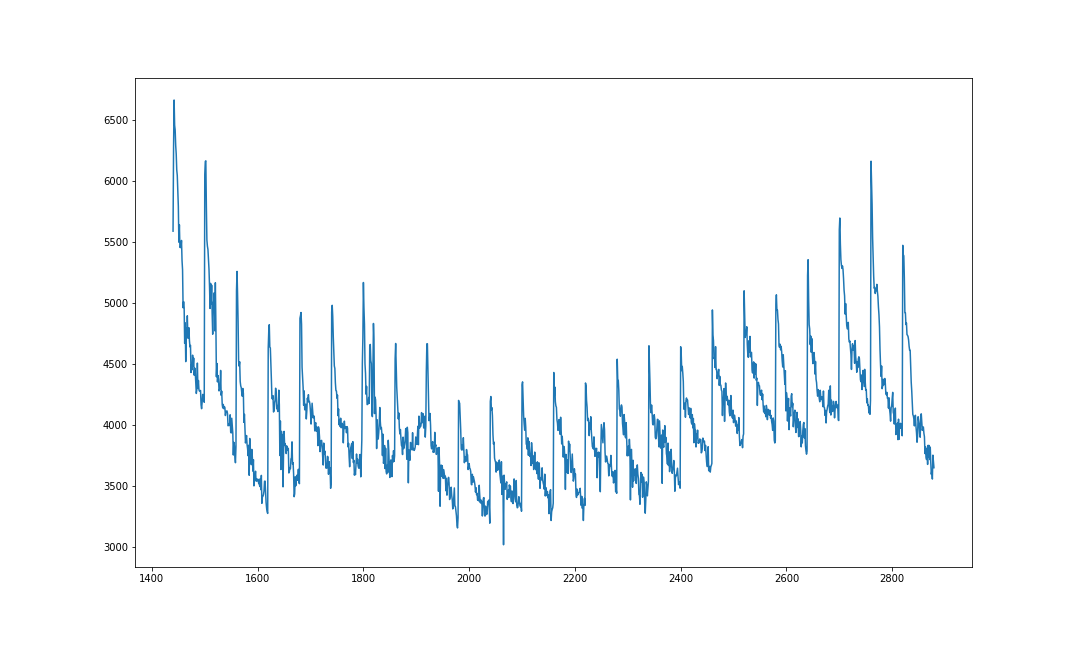
\includegraphics[scale=0.10]{images/008_case_1}
     \end{figure}
	
\end{frame}


\begin{frame}
    \frametitle{Airpush cases. Fraud elimination}
    \begin{itemize}
    	\item Goal: to be able to find such apps automatically
	\item We can reach this goal using frequency analysis
    \end{itemize}
    The framework can be described as follows:
   	 \begin{enumerate}
	 \item Apply logarithm to time series to stabilyze amplitude
 	 \item Remove trend (low frequent part) from time series
	 \item Apply Fourier transform to time series
	 \item Estimate the distribution of periodogram values
	 \item Compare distributions of each application with a distribution of white noise (which is exponential) using Kullback–Leibler divergence 
	 \item If divergence $>$ threshold, then application is marked as suspicious
	\end{enumerate}
\end{frame}



\begin{frame}
    \frametitle{Airpush cases. Fraud elimination}
    \framesubtitle{1. Apply logarithm}
    \begin{figure}
	\textbf{Clean application}
	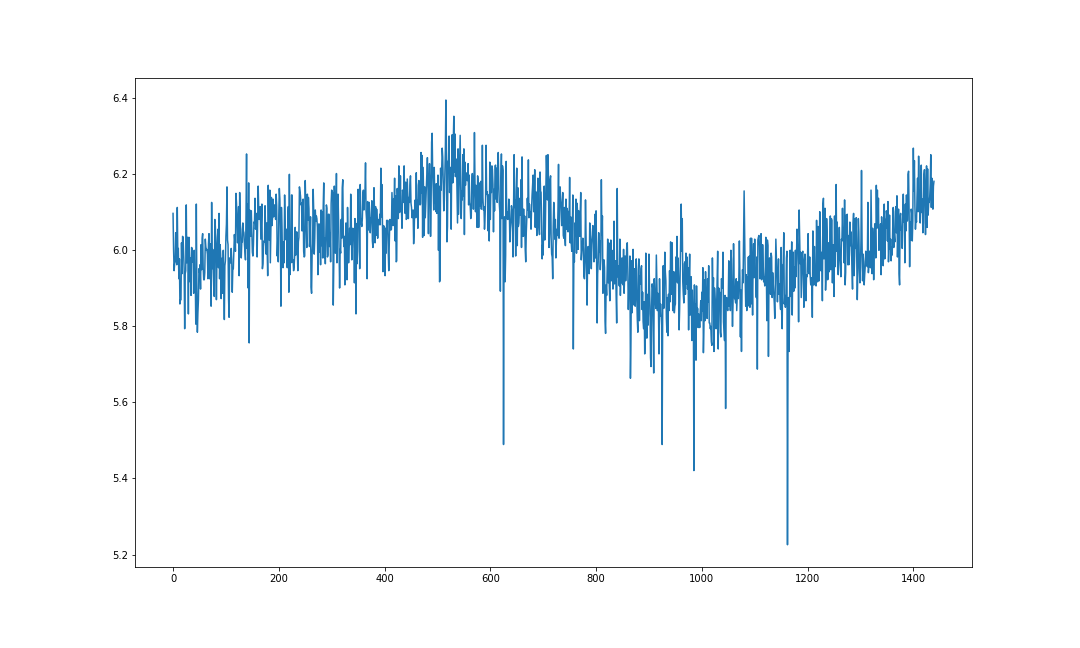
\includegraphics[scale=0.10]{images/009_case_1}
	\textbf{Fraud application}
	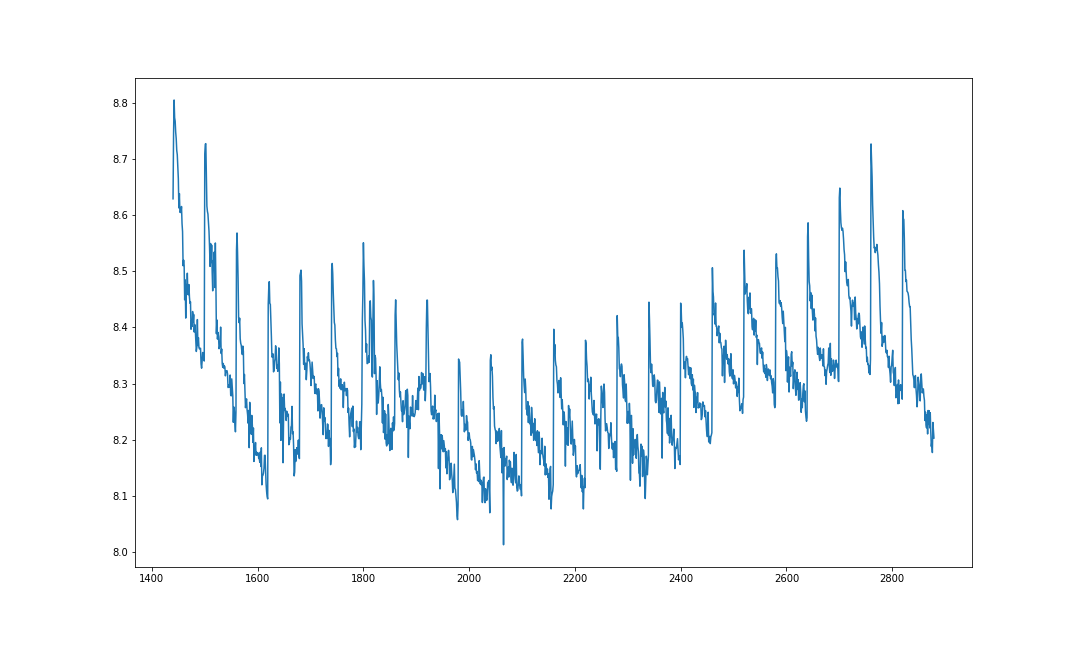
\includegraphics[scale=0.10]{images/010_case_1}
     \end{figure}
\end{frame}

\begin{frame}
    \frametitle{Airpush cases. Fraud elimination}
    \framesubtitle{2. Remove trend}
    \begin{figure}
	\textbf{Clean application}
	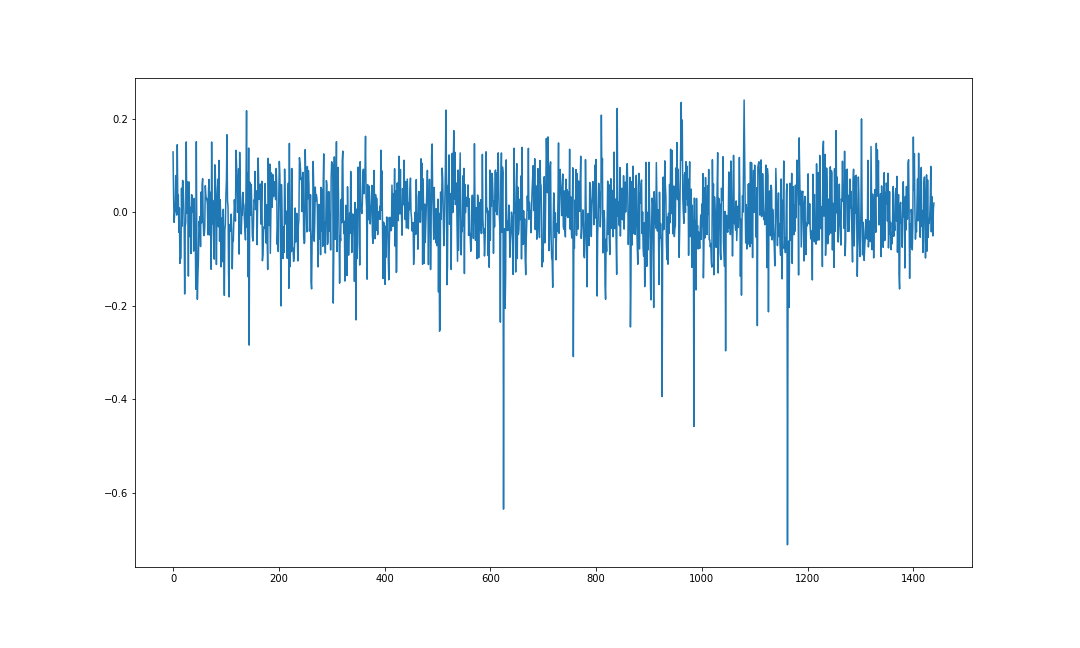
\includegraphics[scale=0.10]{images/011_case_1}
	\textbf{Fraud application}
	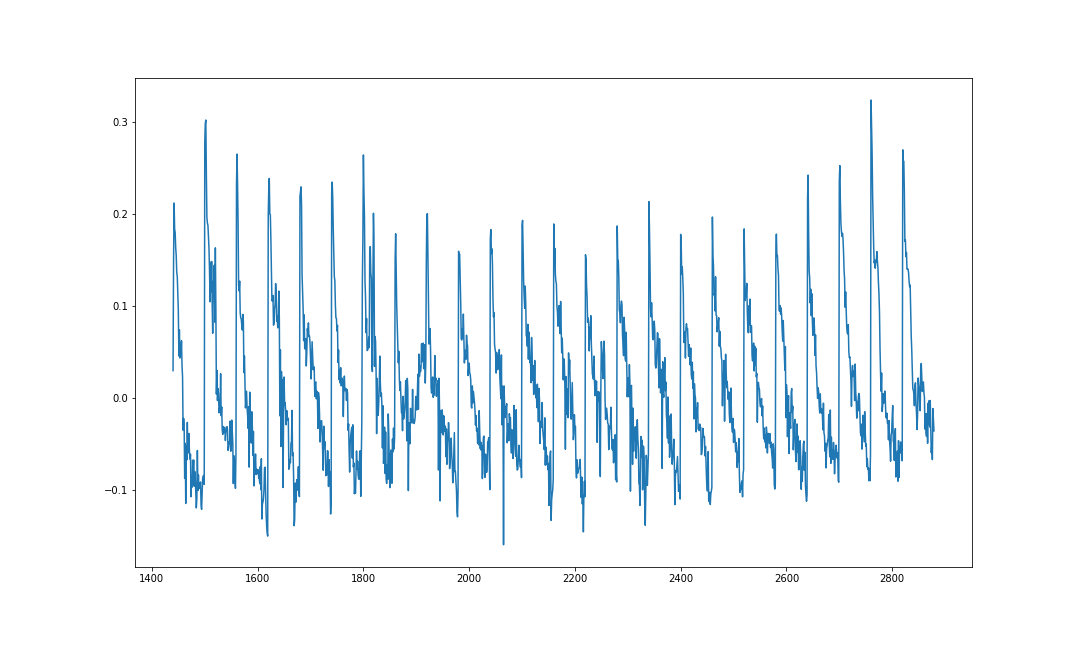
\includegraphics[scale=0.10]{images/012_case_1}
     \end{figure}
\end{frame}

\begin{frame}
    \frametitle{Airpush cases. Fraud elimination}
    \framesubtitle{3. Apply Fourier transform}
    \begin{figure}
	\textbf{Clean application}
	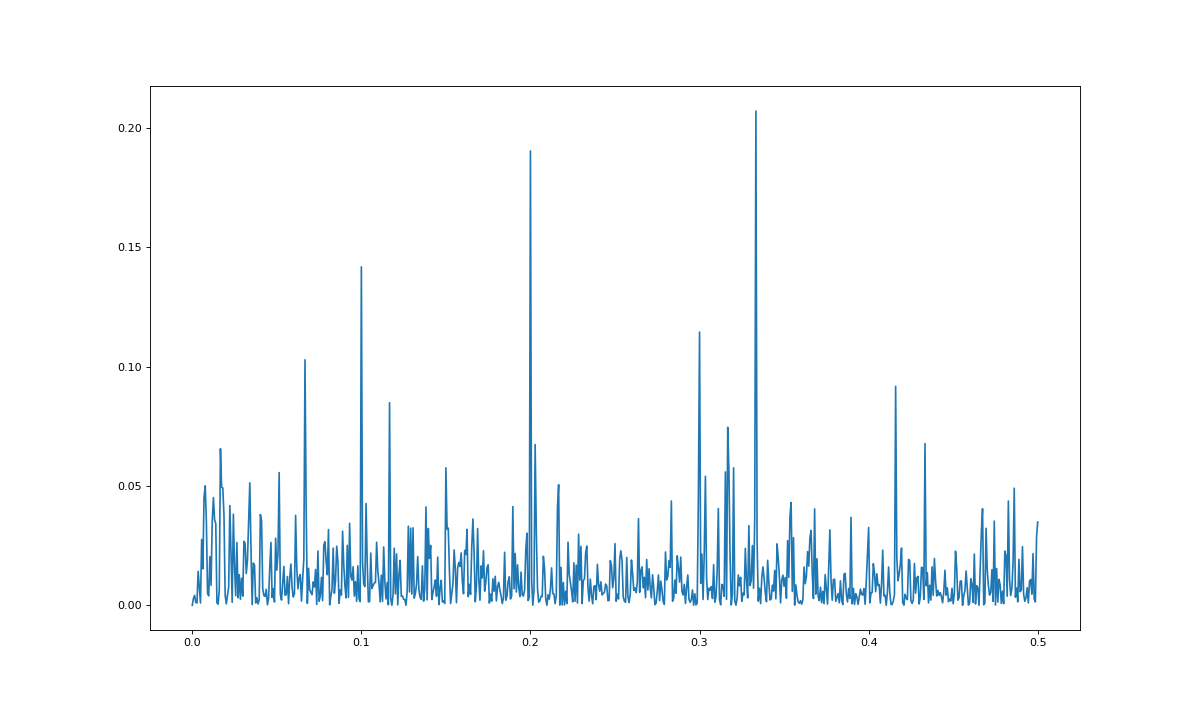
\includegraphics[scale=0.10]{images/013_case_1}
	\textbf{Fraud application}
	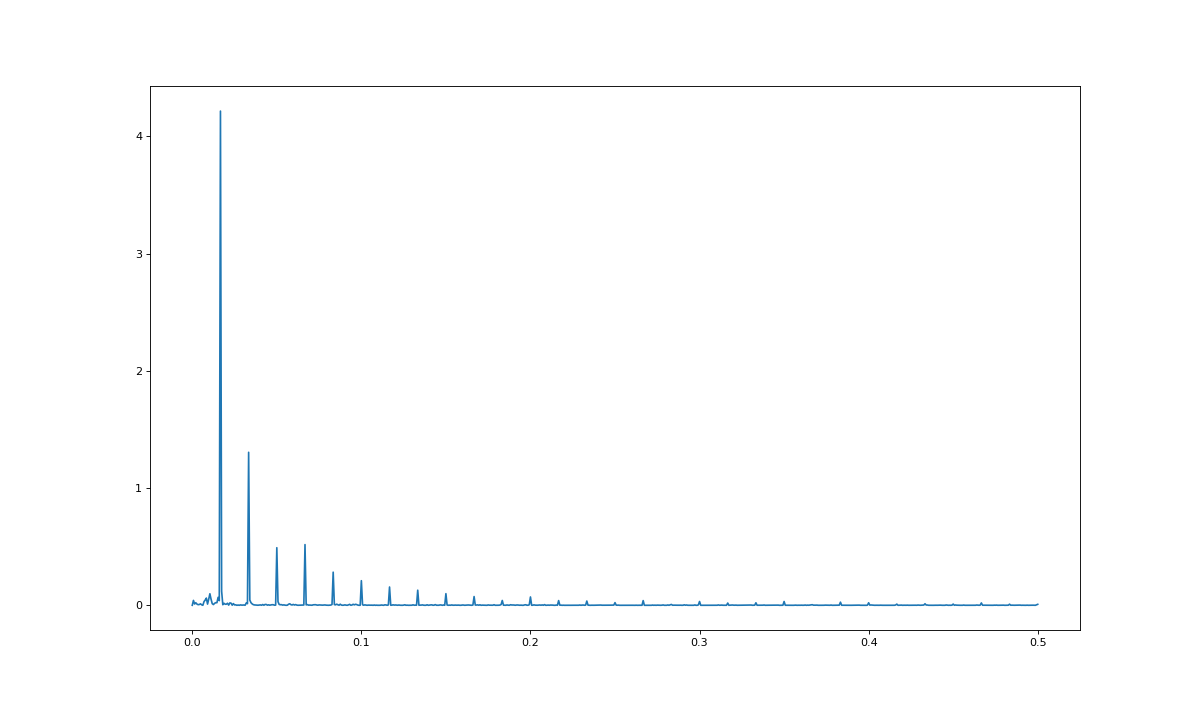
\includegraphics[scale=0.10]{images/014_case_1}
     \end{figure}
\end{frame}

\begin{frame}
    \frametitle{Airpush cases. Fraud elimination}
    \framesubtitle{4. Estimate the distribution of periodogram values}
    \begin{figure}
	\textbf{Clean application}
	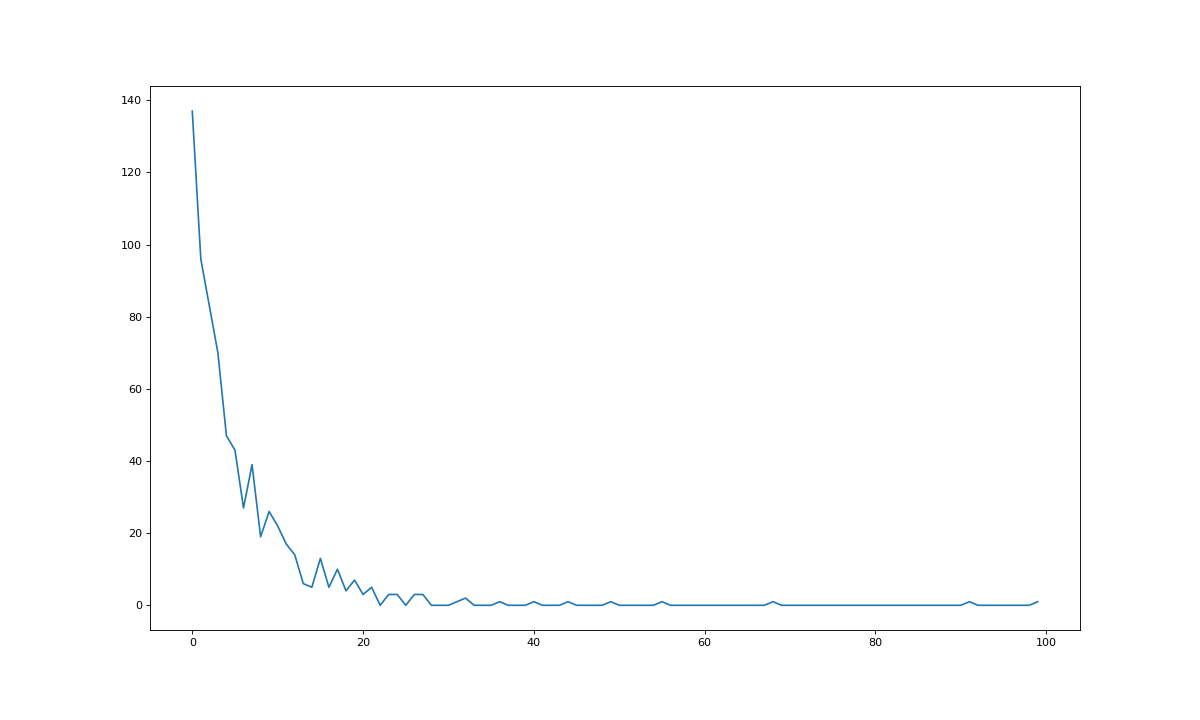
\includegraphics[scale=0.10]{images/015_case_1}
	\textbf{Fraud application}
	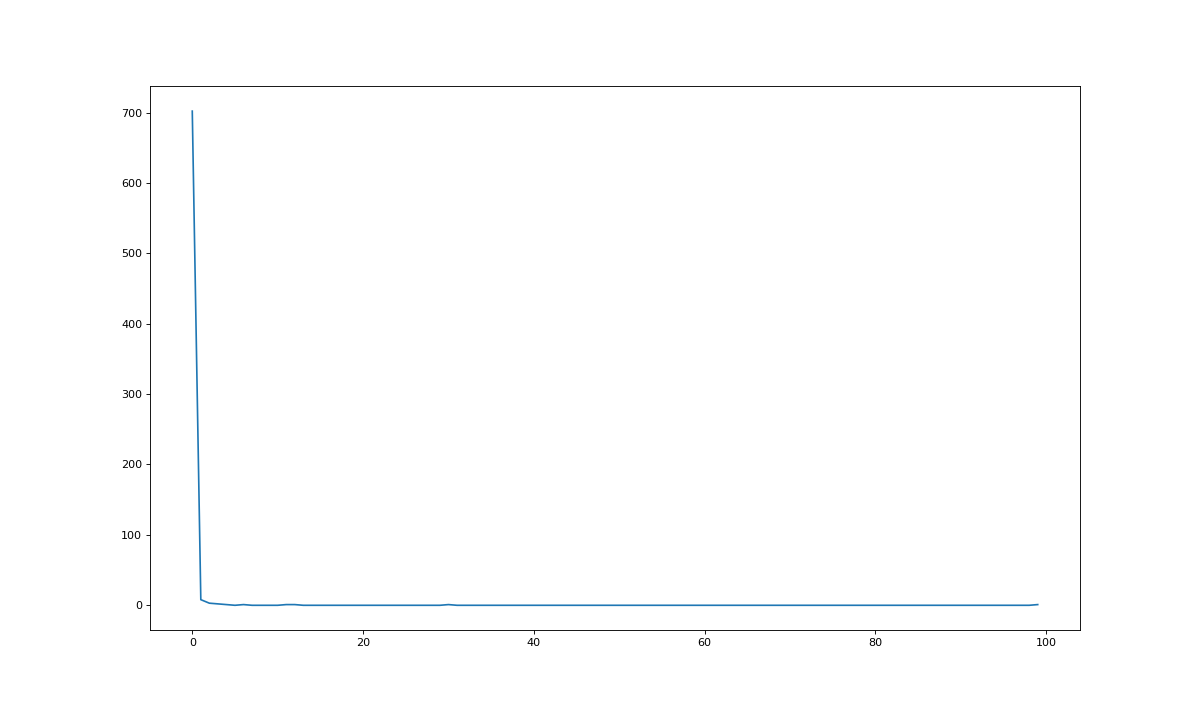
\includegraphics[scale=0.10]{images/016_case_1}
     \end{figure}
\end{frame}

\begin{frame}
    \frametitle{Airpush cases. Fraud elimination}
    \framesubtitle{5. Compare distributions}
    \begin{itemize}
    	\item Clean app score: 0.09
	\item Fraud app score: 1.87
    \end{itemize}
\end{frame}

\end{document}
